% !TEX root = ../thesis.tex

\chapter{Analytická časť}

In most eukaryotic and prokaryotic organisms the hereditary material is either linear double-stranded DNA (deoxyribonucleic acid) molecules or a circular double-stranded DNA molecule. However, some extracellular life forms, might use RNA (ribonucleic acid) as the building block for their genome. For instance, viruses have a genome composed of either single-stranded DNA, double-stranded DNA or RNA, depending on the type of a virus. Therefore, a genome itself, is the complete content of genetic information in an organism, or in other words, all the unique DNA or RNA sequences the organism possesses. 
\section{Nucleotides}

Both of DNA and RNA  are polymeric molecules, that are composed of linear chains of various combinations of four different subunits, called nucleotides. The nucleotide itself is the basic unit of the DNA and RNA molecules, the monomer, which, however, could be found in the cell not only as the bearer of the genetic information, but also as a carrier of energy used to power enzymatic reactions. A five-carbon-atom sugar, a phosphate group and a nitrogenous base are three distinct components which, combined together, make up the quite complex nucleotide molecule. The combination of sugar and base is called a nucleoside, while the phosphate-sugar-base is termed a nucleotide. The nucleotide bases can be either a single-ringed pyrimidine or a double-ringed purine. Dinucleotide, trinucleotide and polynucleotide are the terms corresponding to two, three or many nucleotides connected with each other respectively.

\begin{figure}[!ht]
	\centering
	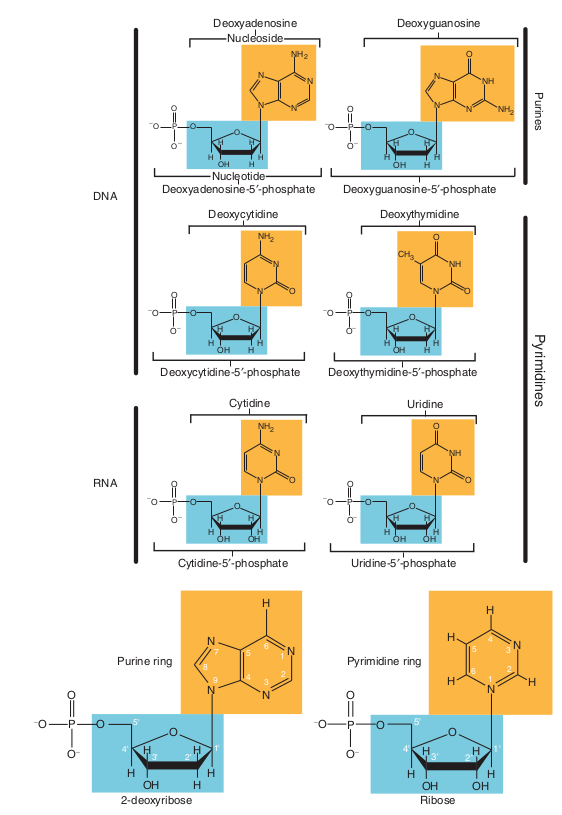
\includegraphics[width=.9\textwidth]{figures/bases}
	\caption{The structures of the pyrimidines and purines found in DNA and RNA. The sugar groups are highlighted in blue and the nitrogenous bases are highlighted in orange. The atoms of the sugar are numbered from 1 to 5. The atoms of the purine ring are numbered from 1 to 9, while those of the pyrimidine ring are numbered from 1 to 6. \label{o:latex_friendly_zone}}
\end{figure}

A nucleotide can be either a purine or pyrimidine. Guanine (G) and adenine (A)  are the common purines for both of DNA and RNA; the pyrimidine called cytosine (C) is also present in both nucleic acids. However, the pyrimidine uracil (U) is limited only to RNA, being replaced with thymine (T) in DNA. There are merely two base-pair combinations that are permissible – A base-paired with T (U) and C base-paired with G. It happens due to the geometries of the nucleotide bases and relative positions of atoms which participate in the connection. This property makes two sequences of polynucleotides in helix complement. Discrete nucleotides are attached to each other through sugar–phosphate bonds that connect the phosphate group on the 5’ carbon of one nucleotide with the hydroxyl group on the 3’ carbon of another nucleotide. The base pairing between adenine and thymine (uracil) involves two hydrogen bonds, while between cytosine and guanine involves three hydrogen bonds.
\section{Nucleodic acid spatial stucture}

As the three-dimensional structure of a nucleotide is not completely rigid, it is possible for DNA to have various spatial architectures: A-form, B-form, Z-form and the circular one. The position of the base relatively to the five-carbon-atom sugar can be changed by a rotation around the N-glycosidic bond and, in this way, significantly affect the three dimensional configuration of the molecule and helix consequently.

\begin{table}[!ht]
	\caption{DNA double helix}\label{t:1}
	\smallskip
	\centering
	
	\begin{tabular}{ |p{3cm}||p{3cm}|p{3cm}|p{3cm}|  }
		\hline
		\multicolumn{4}{|c|}{Features of the different conformations of the DNA double helix} \\
		\hline
		Feature& B-DNA & A-DNA & Z-DNA\\
		\hline
		\hline
		Type of helix & Right-handed & Right-handed & Left-handed\\
		\hline
		Number of base pairs per turn & 10 & 11 & 12\\
		\hline
		Distance between base pairs (nm) & 0.34 & 0.29 & 0.37\\
		\hline
		Distance per complete turn (nm) & 3.4 & 3.2 & 4.5\\
		\hline
		Diameter (nm) & 2.37 & 2.55 & 1.84\\
		\hline
		Major groove & Wide, deep & Narrow, deep & Flat\\
		\hline
		Minor groove & Narrow, shallow & Wide shallow & Narrow, deep\\
		\hline
	\end{tabular}
\end{table}

Moreover, although usually single-stranded, some RNA sequences have the ability to form a double helix. However, double helix RNA is rare and has nothing in common with the genome itself, since only the single-stranded RNA molecules appear to participate in some genome related processes in the eukaryotic and prokaryotic organisms. Since circular DNA may exist in several forms including single-stranded c-DNA, intact double-stranded c-DNA (closed circles with both strands covalently linked), nicked ds-c-DNA (only one strand covalently linked) and “concatenated circles” their properties are not described in the following table.

\section{Chromosomes in eukaryotic genomes}

In eukaryotic cells nucleic acid is situated in a membrane-bound organelle called the nucleus.\footnote{F RANCA , L. T. – C ARRILHO , E. – K IST , T. B. A review of DNA sequencing techniques.
Quarterly reviews of biophysics. 2002, 35, 02, s. 169–200}  The nuclear genome is split into a set of linear double-helix DNA molecules, each contained in a chromosome. No exceptions to this pattern are known: all eukaryotes that have been studied have at least two chromosomes and the DNA molecules are always linear. The only variability at this level of organization of eukaryotic genome is coherent with the number of chromosomes. Moreover, it appears, that biological features of an organism have no dependence on the number of chromosomes. 

\begin{figure}[!ht]
	\centering
	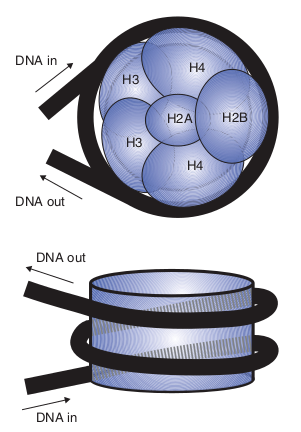
\includegraphics[width=.5\textwidth]{figures/nucleoDetailed}
	\caption{The nucleosome structure. H2A, H2B, H3 and H4 represent different types of histones. \label{o:latex_friendly_zone}}
\end{figure}

Despite the size of a nucleus (5-10 um), an overall length of DNA in the human cell is approximately 2.1m and can be packed inside the cell because of the method the nucleic acid is stored. The genetic material in viruses and bacteria consists of strings of DNA or RNA almost devoid of proteins. However, in eukaryotes, a substantial quantity of protein is associated with the DNA to form chromatin. At the lowest level, the DNA is organized by wrapping DNA strands around he proteins called histones, that contain a large amount of positively charged amino acids arginine and lysine. Those amino acids, and histones in general, play the crucial structural role, making it possible to bind the negative charged phosphate groups of the DNA nucleotides.

Averagely, the DNA rolled around the histones consists of 140-150 base pair, dependently on the species. Such a complex of DNA and histones is termed a nucleosome. These nucleosomes can be further coiled into increasingly larger coils up until forming chromosomes\footnote{C HAISSON , M. J. – P EVZNER , P. A. Short read fragment assembly of bacterial genomes.
Genome research. 2008, 18, 2, s. 324–330.}. However, tight coiling of DNA limits cells ability to access DNA and to process it.\footnote{Analysis of Genes
and Genomes Richard J. Reece University of Manchester, UK} Instead of being constantly coiled, the nucleic acid is usually found in a state called chromatin where some segments of acid are tightly reeled (heterochromatin), while other segments are entirely open (euchromatin). Euchromatin DNA is is highly accessible by the molecular complexes used by the cell and therefore is easier to manipulate with. 

The formation of nucleosomes represents the first level of packing, whereby
the DNA is reduced to about one-third of its original length. In the nucleus,
however, chromatin does not exist in this extended form.\footnote{Kipling, D. and Cooke, H.J. 1990. Hypervariable ultra-long telomeres in
mice. Nature 374: 400–402} Instead, the 10
nm chromatin fibre is further packed into a thicker 30 nm fibre, which was
originally called a solenoid. It is not clear whether the transition between the
10 nm fibre and the 30 nm fibre represents a physiological event or whether it
merely occurs in vitro as a consequence of altering the salt concentration. The
30 nm fibre does, however, consist of numerous nucleosomes packed closely
together, but the precise orientation and details of the structure are not clear.\footnote{Greider, C.W. 1996. Telomere length regulation. Annu. Rev. Biochem.
65: 337–365.}

The amount and extent of packing are determined by a sell, to control which sections of the genome can be expressed and which cannot. It affects cellular function and appears to be the predominant cause of differentiating cells type, while having the same DNA.

\begin{figure}[!ht]
	\centering
	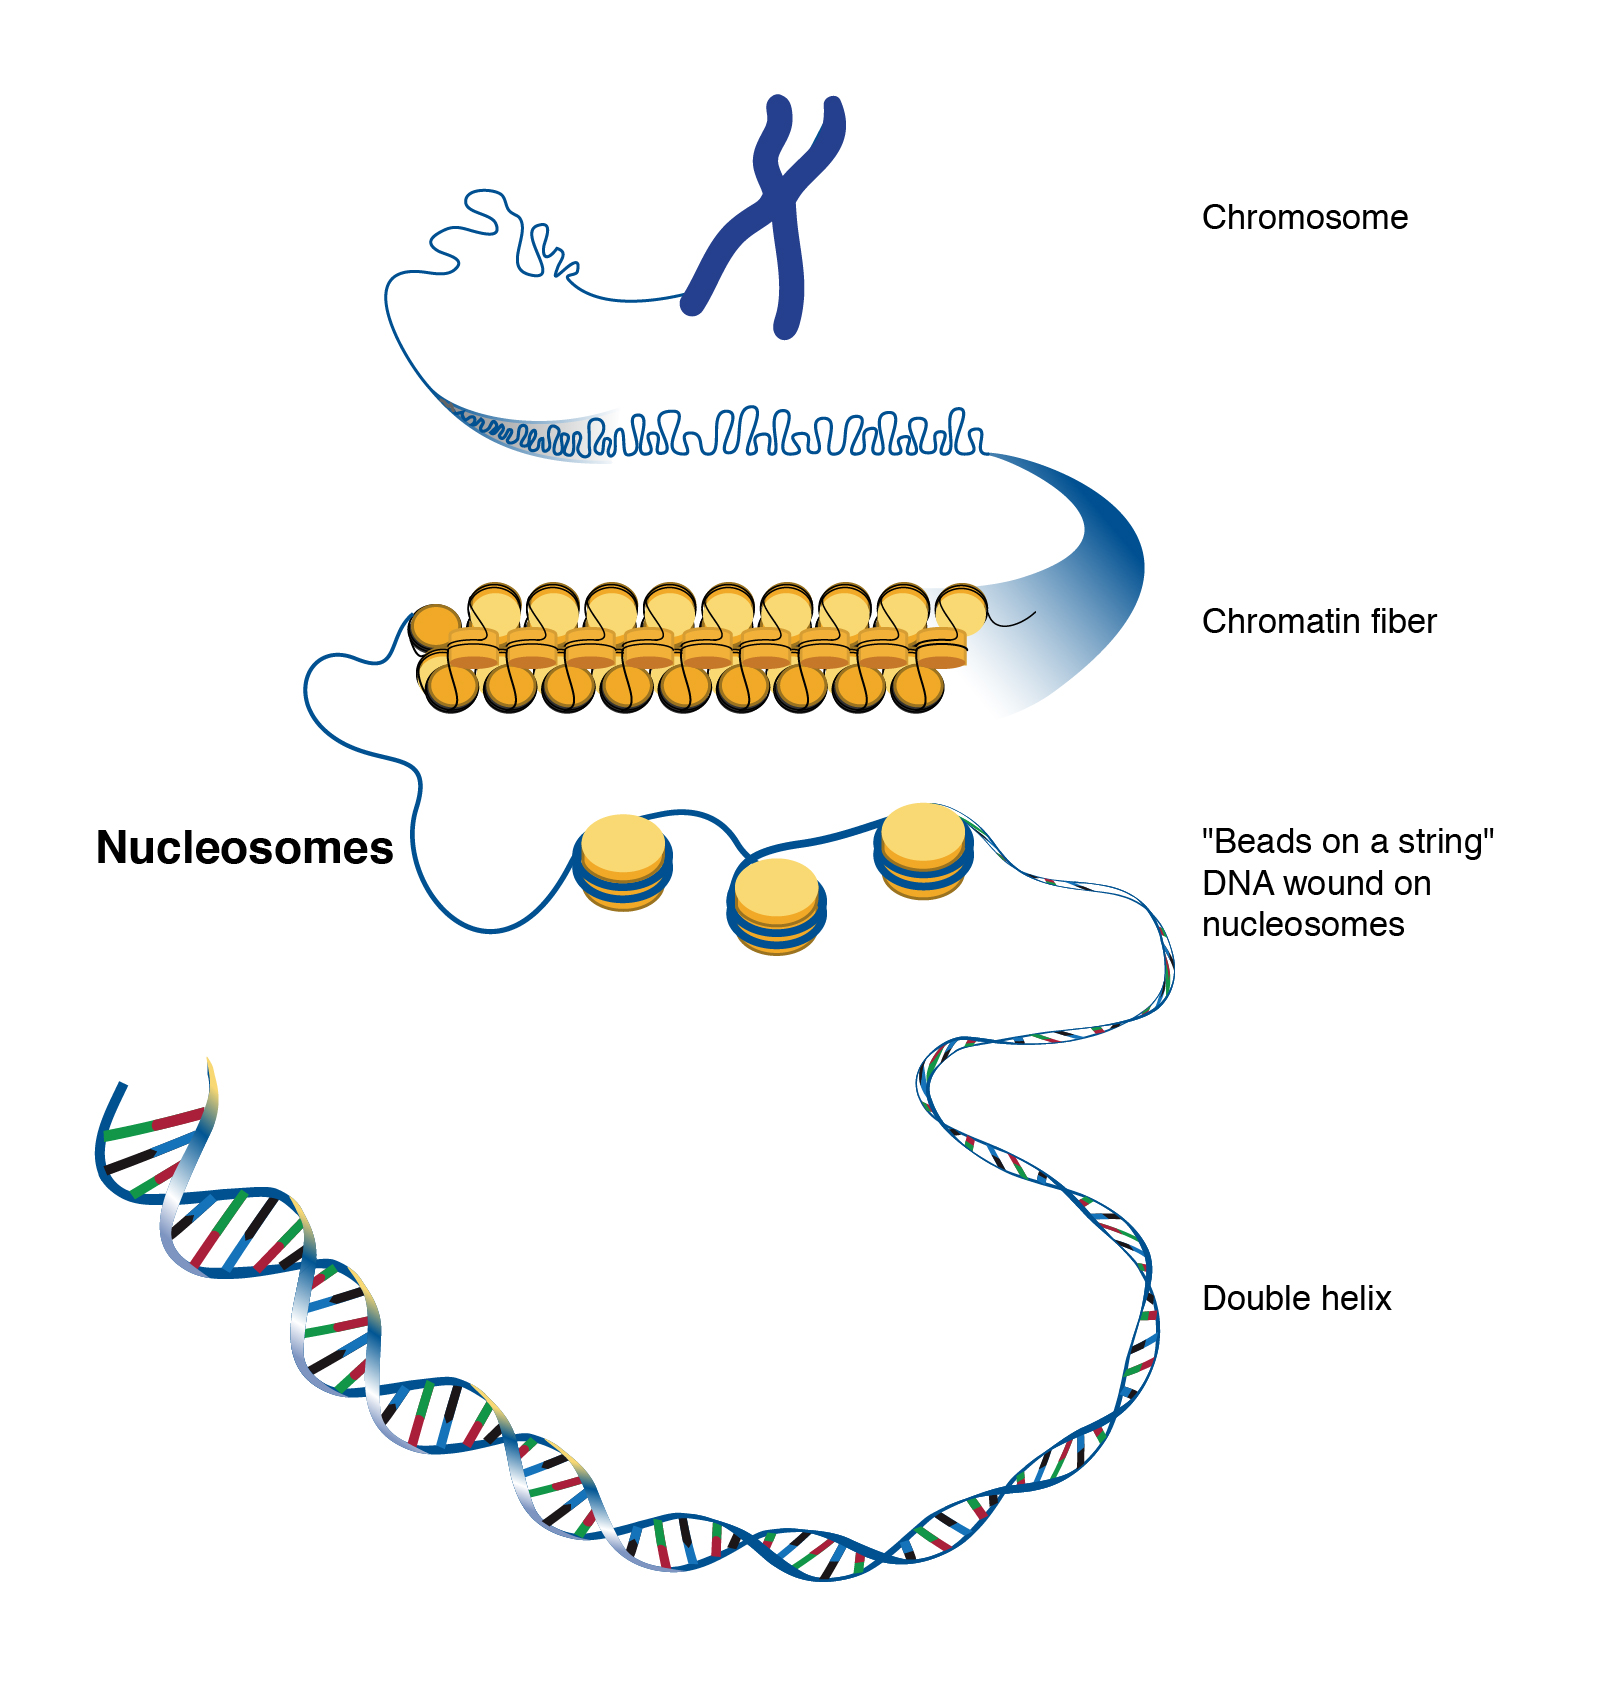
\includegraphics[width=.9\textwidth]{figures/nucleosome1}
	\caption{Ncleosomes as the part of a chromosome.\label{o:latex_friendly_zone}}
\end{figure}

Transcription is the process by which an RNA copy of one of the strands in
the DNA double helix is made. The antisense strand of the DNA directs the
synthesis of a complementary RNA molecule. The RNA molecule produced is
therefore identical to the sense strand of the DNA – except that it contains U
instead of T. There are fundamental differences in the ways in which genes are
transcribed in prokaryotes and eukaryotes.\footnote{Smogorzewska, A. and de Lange, T. 2004. Regulation of telomerase by
telomeric proteins. Annu. Rev. Biochem. 73: 177–208} Here, it is important to understand
the processes involved in each case. Many of the experiments we will look at
in later chapters involve the use of eukaryotic cells, but the bacterium E. coli
still plays a vital role in almost all genetic engineering experiments.
Transcription begins at specific DNA sequences called promoters. Like DNA
replication, transcription occurs in three phases – initiation, elongation and
termination. Initiation of transcription usually occurs to the 3 side of the
promoter, and termination occurs at specific sites downstream of the coding
sequence of the gene. At first glance, the overall architecture of a typical
prokaryotic gene and a typical eukaryotic gene may appear to be similar. However, the controlling region for eukaryotic genes will not
function in a prokaryotic cell, and vice versa.\footnote{Levis, R.W. 1989. Viable deletions of a telomere from a Drosophila
chromosome. Cell 58: 791–801.}
Most protein coding genes in prokaryotes are transcriptionally active by
default. That is to say, in the absence of other factors, the RNA polymerase can
recognize the promoter of a gene, bind to it and produce RNA. Transcriptional
control is brought to bear on the gene by repressor proteins that bind to DNA
sequences adjacent to the RNA polymerase binding site. DNA binding by the
repressor either occludes RNA polymerase binding and/or prevents a bound
polymerase from transcribing. The eukaryotic RNA polymerase involved in the
production of protein coding genes is unable to recognize promoter
sequences on its own. Therefore, eukaryotic genes are transcriptionally inactive
in the absence of other factors. In both prokaryotes and eukaryotes, transcrip-
tion is a highly regulated process. Proper timing and levels of gene expression
are essential to almost all cellular processes.